\documentclass[a4paper,UTF8]{article}
\usepackage{ctex}
\usepackage[margin=1.25in]{geometry}
\usepackage{color}
\usepackage{graphicx}
\usepackage{amssymb}
\usepackage{amsmath}
\usepackage{amsthm}
\usepackage{enumerate}
\usepackage{bm}
\usepackage{hyperref}
\usepackage{epsfig}
\usepackage{color}
\usepackage{mdframed}
\usepackage{lipsum}
\usepackage{mathtools}
\usepackage{hyperref}
\usepackage{diagbox}
\usepackage{float}
\usepackage{caption}
\usepackage{algorithm}
\usepackage{algorithmicx}  
\usepackage{algpseudocode}
\usepackage{amsmath} 
\usepackage{graphicx}
\usepackage{subfigure}
\usepackage{url}
\newmdtheoremenv{thm-box}{myThm}
\newmdtheoremenv{prop-box}{Proposition}
\newmdtheoremenv{def-box}{定义}
\usepackage{listings}
\usepackage{xcolor}
\lstset{
	numbers=left, 
	numberstyle= \tiny, 
	keywordstyle= \color{ blue!70},
	commentstyle= \color{red!50!green!50!blue!50}, 
	frame=shadowbox, % 阴影效果
	rulesepcolor= \color{ red!20!green!20!blue!20} ,
	escapeinside=``, % 英文分号中可写入中文
	xleftmargin=2em,xrightmargin=2em, aboveskip=1em,
	framexleftmargin=2em
} 

\usepackage{booktabs}

\setlength{\evensidemargin}{.25in}
\setlength{\textwidth}{6in}
\setlength{\topmargin}{-0.5in}
\setlength{\topmargin}{-0.5in}

% \setlength{\textheight}{9.5in}
%%%%%%%%%%%%%%%%%%此处用于设置页眉页脚%%%%%%%%%%%%%%%%%%
\usepackage{fancyhdr}                                
\usepackage{lastpage}                                           
\usepackage{layout}                                             
\footskip = 10pt 
\pagestyle{fancy}                    % 设置页眉                 
\lhead{研一下学期}                    
\chead{论文阅读笔记}                                                
% \rhead{第\thepage/\pageref{LastPage}页} 
\rhead{Step8}                                                                                               
\cfoot{\thepage}                                                
\renewcommand{\headrulewidth}{1pt}  			%页眉线宽,设为0可以去页眉线
\setlength{\skip\footins}{0.5cm}    			%脚注与正文的距离           
\renewcommand{\footrulewidth}{0pt}  			%页脚线宽,设为0可以去页脚线

\makeatletter 									%设置双线页眉                                        
\def\headrule{{\if@fancyplain\let\headrulewidth\plainheadrulewidth\fi%
\hrule\@height 1.0pt \@width\headwidth\vskip1pt	%上面线为1pt粗  
\hrule\@height 0.5pt\@width\headwidth  			%下面0.5pt粗            
\vskip-2\headrulewidth\vskip-1pt}      			%两条线的距离1pt        
 \vspace{6mm}}     								%双线与下面正文之间的垂直间距              
\makeatother  

%%%%%%%%%%%%%%%%%%%%%%%%%%%%%%%%%%%%%%%%%%%%%%
\numberwithin{equation}{section}
%\usepackage[thmmarks, amsmath, thref]{ntheorem}
\newtheorem{theorem}{Theorem}
\newtheorem*{definition}{Definition}
\newtheorem*{solution}{Solution}
\newtheorem*{prove}{Proof}
\newcommand{\indep}{\rotatebox[origin=c]{90}{$\models$}}

\usepackage{multirow}

%--

%--
\begin{document}
\title{论文阅读笔记\\
Step8}
\author{MF1833063, 史鹏, spwannasing@gmail.com}
\maketitle

\newpage
\section{SEMI-SUPERVISED CLASSIFICATION WITH GRAPH CONVOLUTIONAL NETWORKS}
本文提出了一种图卷积网络(graph covolutional networks, GCNs),该网络是传统卷积算法在图结构数据上的一个变体,可以直接用于处理图结构数据。从本质上讲,GCN 是谱图卷积(spectral graph convolution) 的局部一阶近似(localized first-order approximation)。GCN的另一个特点在于其模型规模会随图中边的数量的增长而线性增长。总的来说,GCN 可以用于对局部图结构与节点特征进行编码。
\begin{figure}[H]
	\centering
	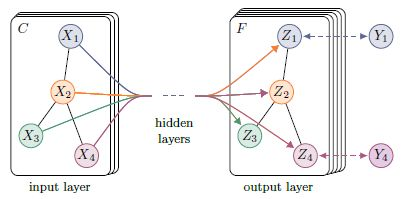
\includegraphics[width=\textwidth]{1-1.jpg}
\end{figure}
图卷积神经网络的(单层)最终形式:
$H^{(l+1)}=\sigma\left(\tilde{D}^{-\frac{1}{2}} \tilde{A} \tilde{D}^{-\frac{1}{2}} H^{(l)} W^{(l)}\right)$

\newpage
\section{Semantic-Unit-Based Dilated Convolution for Multi-Label Text Classification}
本文是基于seq2seq的多标签文本分类在attention上的一些改进工作。主要贡献有两点:

1.提出了所谓的“语义单元”,因为在多标签文本分类中,word-level的作用没有那么大,而是“semantic units”来决定文本的分类。

2.使用了Hybrid Attention将semantic units和word level的attention混合起来。

\begin{figure}[H]
	\centering
	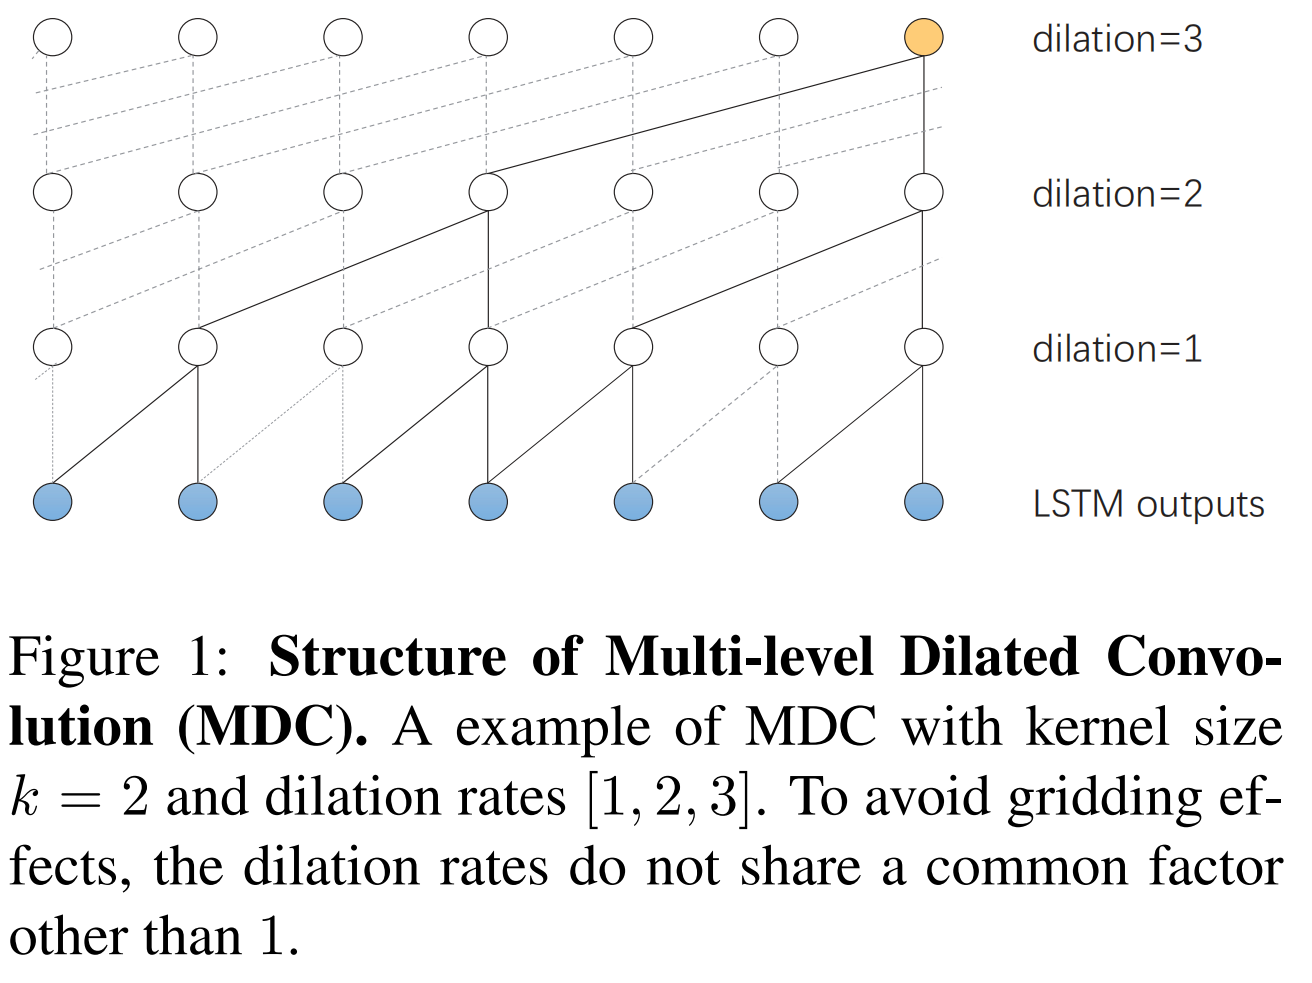
\includegraphics[width=0.6\textwidth]{2-1.png}
\end{figure}

\begin{figure}[H]
	\centering
	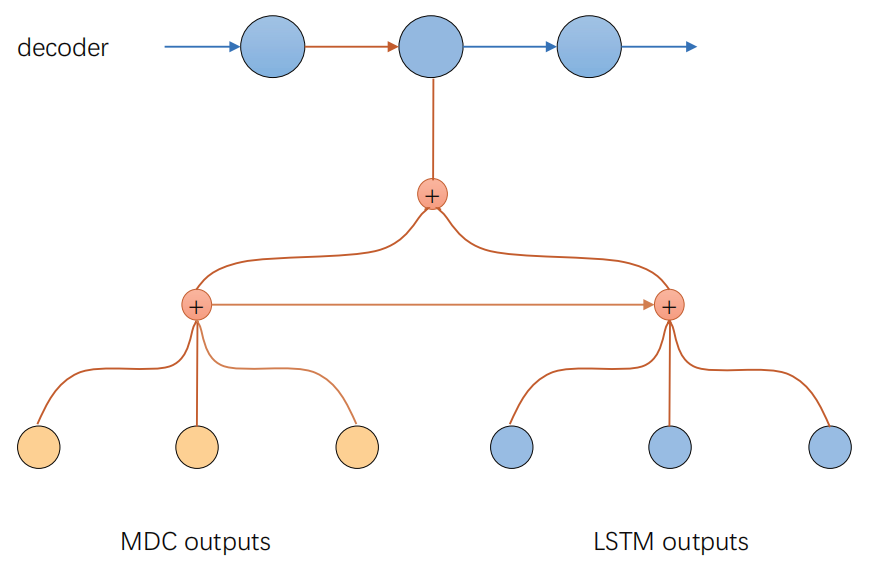
\includegraphics[width=0.6\textwidth]{2-2.png}
	\caption{Structure of Hybrid Attention.}
\end{figure}

\newpage
\section{A Deep Reinforced Sequence-to-Set Model for Multi-Label Classification}
本文的主要Motivation是解决多标签文本分类中Seq2Seq模型的输出序列的顺序问题,因为label之间本来应该是无序的,即交换不变性,
这里所做的工作则是提出用强化学习来解决label之间的顺序问题,reward即为预测label序列和答案之间的F1值。
\begin{equation}
	\mathcal{L}(\theta)=-\mathbb{E}_{\boldsymbol{y} \sim p_{\theta}}[r(\boldsymbol{y})]
	\end{equation}
	\begin{equation}
		\nabla_{\theta} \mathcal{L}(\theta) \approx-\left[r\left(\boldsymbol{y}^{s}\right)-r\left(\boldsymbol{y}^{g}\right)\right] \nabla_{\theta} \log \left(p_{\theta}\left(\boldsymbol{y}^{s}\right)\right)
		\end{equation}
		\begin{equation}
			r(\boldsymbol{y})=\mathrm{F}_{1}\left(\boldsymbol{y}, \boldsymbol{y}^{*}\right)
			\end{equation}
其它的结构基本一致。

\section{Compositional Questions Do Not Necessitate Multi-hop Reasoning}
这篇文章主要是提出了在HotPotQA数据集中存在的一个问题:所谓的multi-hop其实不是必要的,大多数问题可以在只提供sigle paragraph的情况下就正确的回答出来。
然后提出了一个Single-Paragraph QA模型。

分别将paragraph送入Bert
\begin{align}
	S^{\prime}=\mathrm{BERT}(S) \in \mathbb{R}^{h \times(m+n+1)}
	\end{align}
	
	然后选取$y_{\text {empty }}$最小的作为答案输出。

	\begin{align}
		\left[y_{\text {span }} ; y_{\text {yes }} ; y_{\text {no }} ; y_{\text {empty }}\right]=W_{1} \text { maxpool }\left(S^{\prime}\right)
		\end{align}
		\begin{figure}[H]
			\centering
			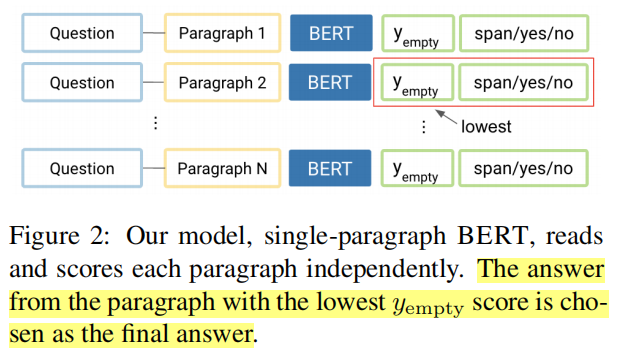
\includegraphics[width=0.6\textwidth]{4-1.png}
		\end{figure}
\end{document}